\clearpage\section{Materiais e montagem}
\begin{table}[H]\centering\small\caption{Componentes empregados no projeto}\label{tab:2}
\rowcolors{2}{tcdlight}{white}\begin{tabularx}{\linewidth}{>{\hsize=0.2969\hsize\linewidth=\hsize\raggedright\arraybackslash}X>{\hsize=1.2062\hsize\linewidth=\hsize\raggedright\arraybackslash}X>{\hsize=1.4969\hsize\linewidth=\hsize\raggedright\arraybackslash}X}
\rowcolor{tcdnavy} \textcolor{white}{\textbf{Qtd.}} & \textcolor{white}{\textbf{Componente}} & \textcolor{white}{\textbf{Função}} \\
2 & ESP32 Dev Module & Processamento e interfaces seriais. \\
2 & Transmissor FS1000A, 433 MHz & Envio de dados e confirmações. \\
2 & Receptor RF 433 MHz & Recepção; modelo exato não confirmado. \\
1 & OLED SSD1306 128\ensuremath{\times}64 I\textsuperscript{2}C & Exibição no circuito B. \\
2 & Protoboards & Montagem dos circuitos. \\
2 & Computadores e cabos USB & Alimentação local, programação e comunicação. \\
4 & Condutores de cabo Ethernet & Antenas artesanais TX e RX. \\
Diversos & Jumpers, ferro de solda, solda & Ligações elétricas e fixação das antenas. \\
\bottomrule\end{tabularx}\end{table}
\begin{figure}[H]\centering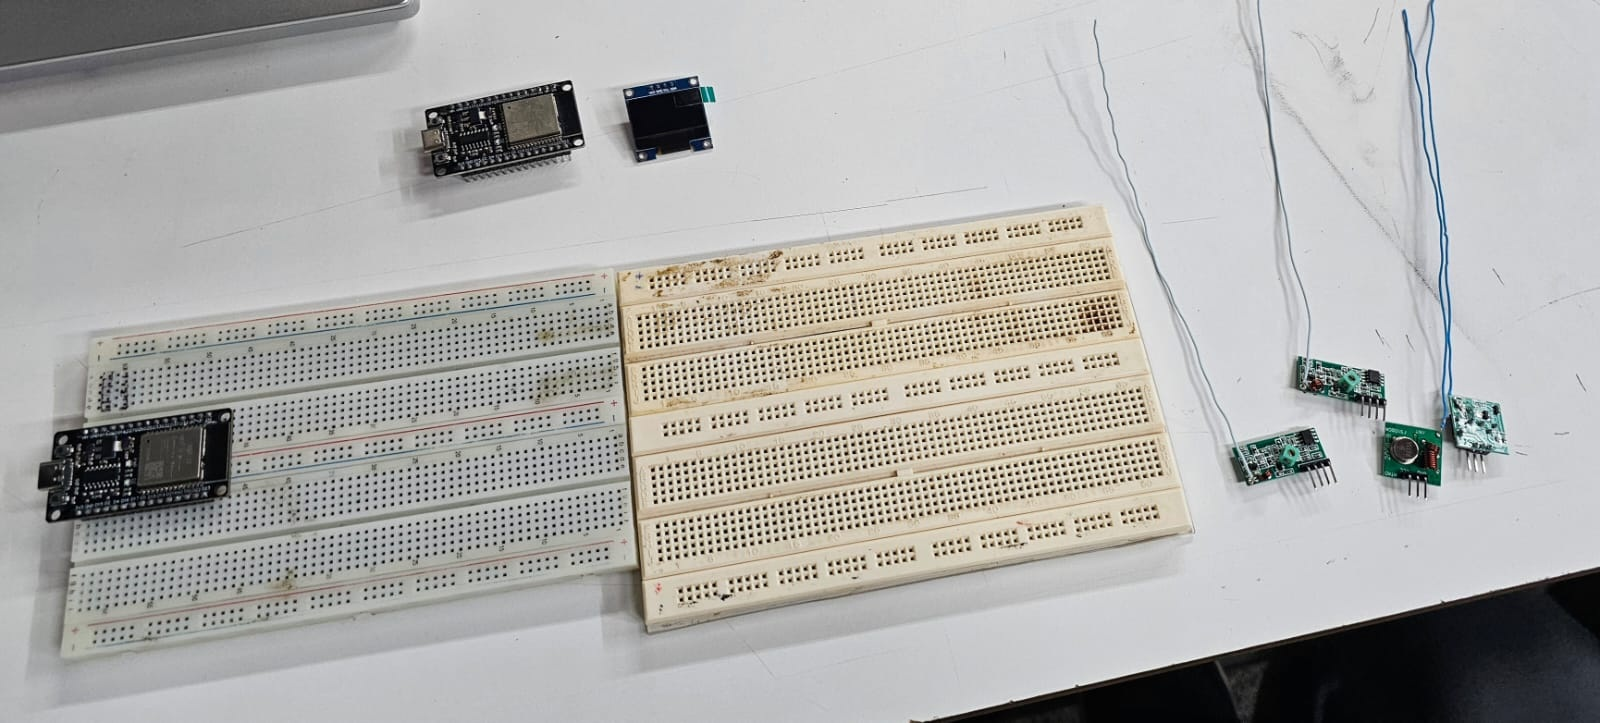
\includegraphics[width=\linewidth,height=180pt,keepaspectratio]{figuras/old_5_1.jpg}\caption{Componentes separados antes da montagem. Fonte: acervo da equipe (2026).}\label{fig:old_5_1}\end{figure}
\setcounter{subsection}{0}\subsection{Preparação elétrica}
Identificar os pinos impressos e as tensões nominais de cada módulo antes de ligar. O VIN/5 V aparece nos desenhos anteriores, mas a compatibilidade do hardware RF deve ser conferida. Os GPIOs do ESP32 não toleram 5 V diretamente; quando a saída DATA do receptor exceder o nível admissível, utilizar adaptação de nível apropriada. Montar com alimentação desligada e testar continuidade, polaridade e ausência de curtos.

\setcounter{subsection}{1}\subsection{Confecção das antenas}
A equipe reaproveitou condutores individuais de um cabo de rede Ethernet. As pontas foram desencapadas e soldadas nos pontos ANT dos módulos. Nos transmissores, o fio foi mantido reto e vertical; nos receptores, o condutor foi enrolado em espiras.

\begin{figure}[H]\centering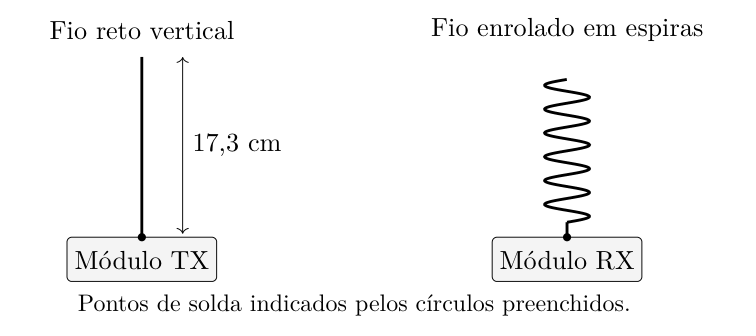
\includegraphics[width=\linewidth,height=135pt,keepaspectratio]{figuras/antenas.png}\caption{Geometria das antenas TX e RX, sem escala. Fonte: relatório técnico anterior.}\label{fig:antenas}\end{figure}
\subsubsection*{Dimensionamento do transmissor}
A antena TX foi confeccionada com comprimento de 17,3 cm, próximo de um quarto do comprimento de onda em espaço livre para 433 MHz:

\textbf{\ensuremath{\lambda} = c/f = 3,0 \ensuremath{\times} 10\textsuperscript{8} / (433 \ensuremath{\times} 10\textsuperscript{6}) \ensuremath{\approx} 0,693 m\\ L = \ensuremath{\lambda}/4 \ensuremath{\approx} 0,173 m = 17,3 cm.}

A antena RX helicoidal reduz a extensão física do fio. O diâmetro, o passo, o comprimento total e a quantidade de espiras não foram padronizados; por isso, não é possível determinar sua ressonância ou ganho a partir das fotos.

\begin{figure}[H]\centering
\begin{minipage}[t]{0.48\linewidth}\centering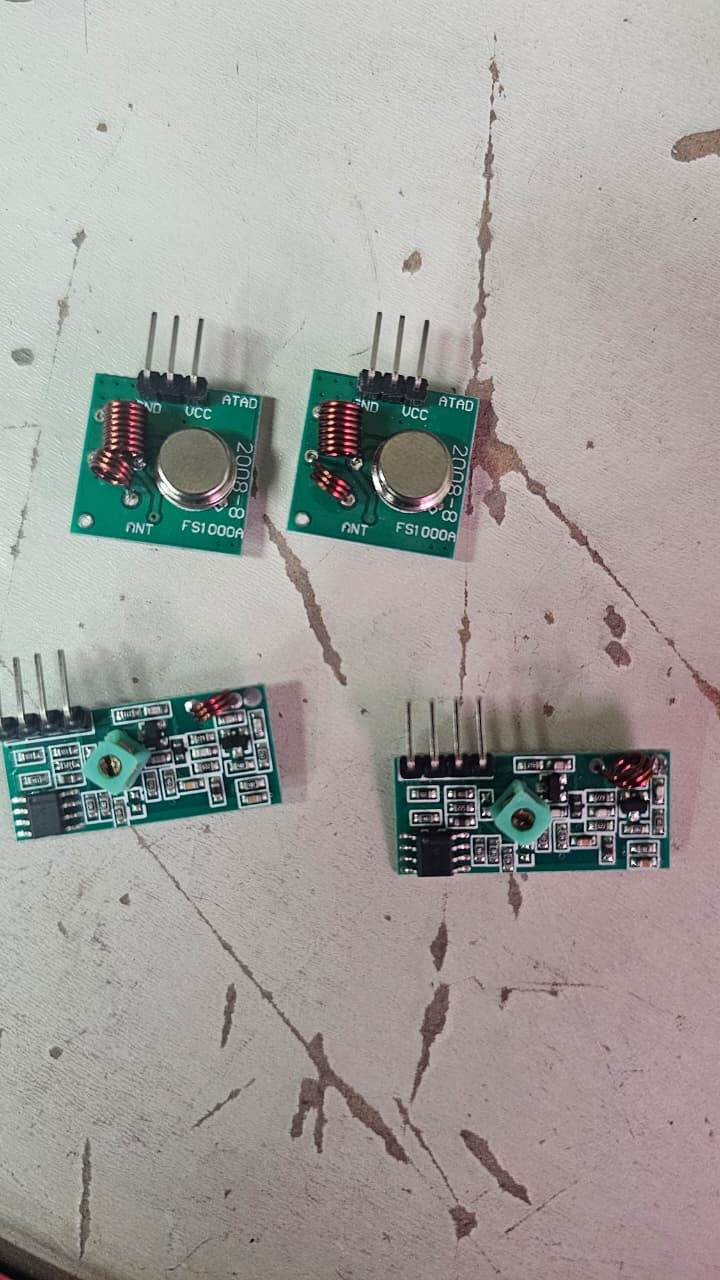
\includegraphics[width=\linewidth,height=150pt,keepaspectratio]{figuras/old_6_1.jpg}\caption{Conjuntos TX/RX utilizados.}\label{fig:old_6_1}\end{minipage}
\hfill
\begin{minipage}[t]{0.48\linewidth}\centering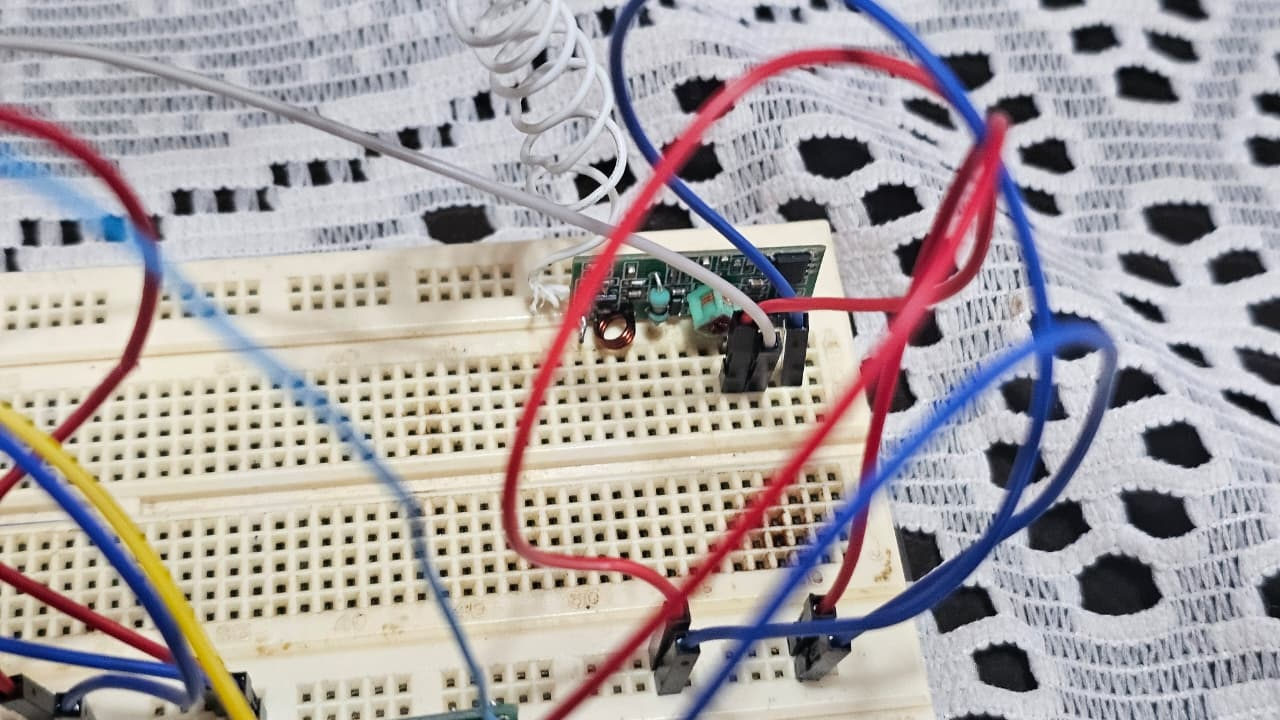
\includegraphics[width=\linewidth,height=150pt,keepaspectratio]{figuras/old_7_1.jpg}\caption{Detalhe da antena RX helicoidal.}\label{fig:old_7_1}\end{minipage}
\end{figure}
{\small Fonte das fotografias: acervo da equipe (2026). Não foram medidos impedância, ganho ou largura de banda. A montagem e a orientação das antenas influenciam o resultado do enlace.\par}
\setcounter{subsection}{2}\subsection{Circuito A — montagem}
\begin{figure}[H]
\centering
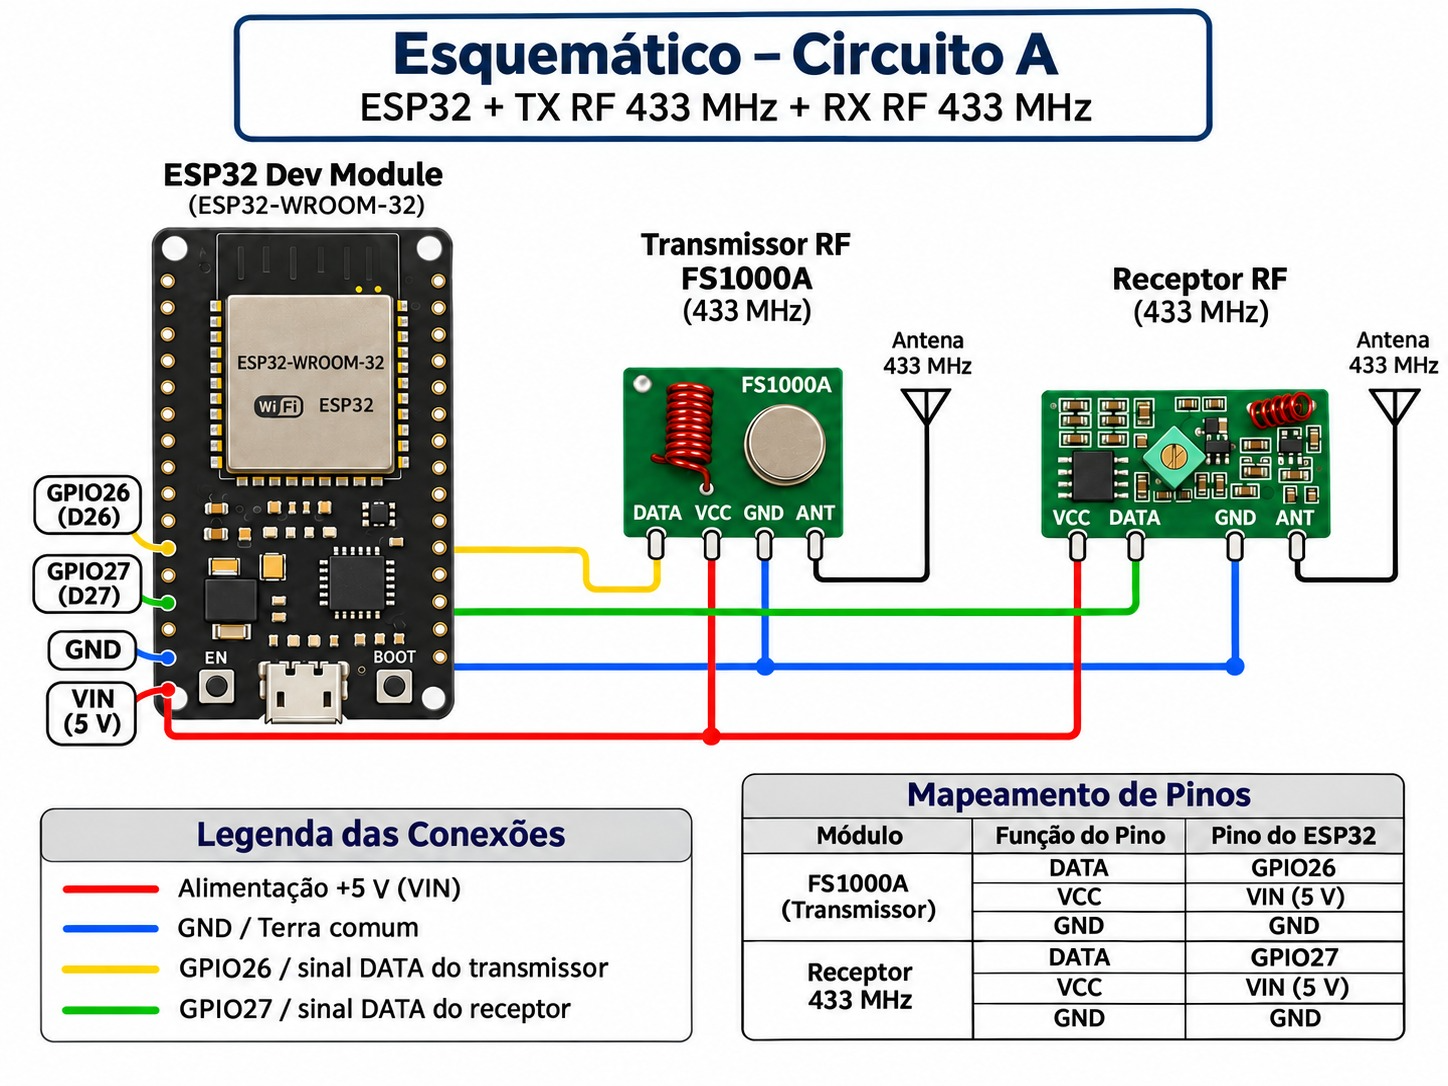
\includegraphics[width=\linewidth,height=225pt,keepaspectratio]{figuras/esq_a.png}
\caption{Esquemático atualizado do Circuito A (ESP32 + transmissor RF 433 MHz + receptor RF 433 MHz). Fonte: elaboração da equipe.}
\label{fig:esq_a}
\end{figure}
\begin{table}[H]\centering\small\caption{Mapeamento das ligações do circuito A}\label{tab:3}
\rowcolors{2}{tcdlight}{white}\begin{tabularx}{\linewidth}{>{\hsize=0.6186\hsize\linewidth=\hsize\raggedright\arraybackslash}X>{\hsize=1.3814\hsize\linewidth=\hsize\raggedright\arraybackslash}X}
\rowcolor{tcdnavy} \textcolor{white}{\textbf{Pino ESP32 A}} & \textcolor{white}{\textbf{Conexão}} \\
GPIO26 & DATA do transmissor RF. \\
GPIO27 & DATA do receptor RF (verificar nível lógico). \\
GND & Terra comum local, TX e RX. \\
Alimentação RF & Conforme tensão nominal dos módulos; verificar VIN/\allowbreak 5 V. \\
\bottomrule\end{tabularx}\end{table}
\begin{enumerate}
\item Posicionar o ESP32 e os módulos TX/RX na protoboard e conectar os terras locais.
\item Soldar as antenas com a montagem desenergizada. Interligar DATA TX ao GPIO26 e DATA RX ao GPIO27.
\item Conferir alimentação e níveis lógicos antes de energizar. Ligar o computador A ao ESP32 por USB.
\end{enumerate}
\begin{figure}[H]\centering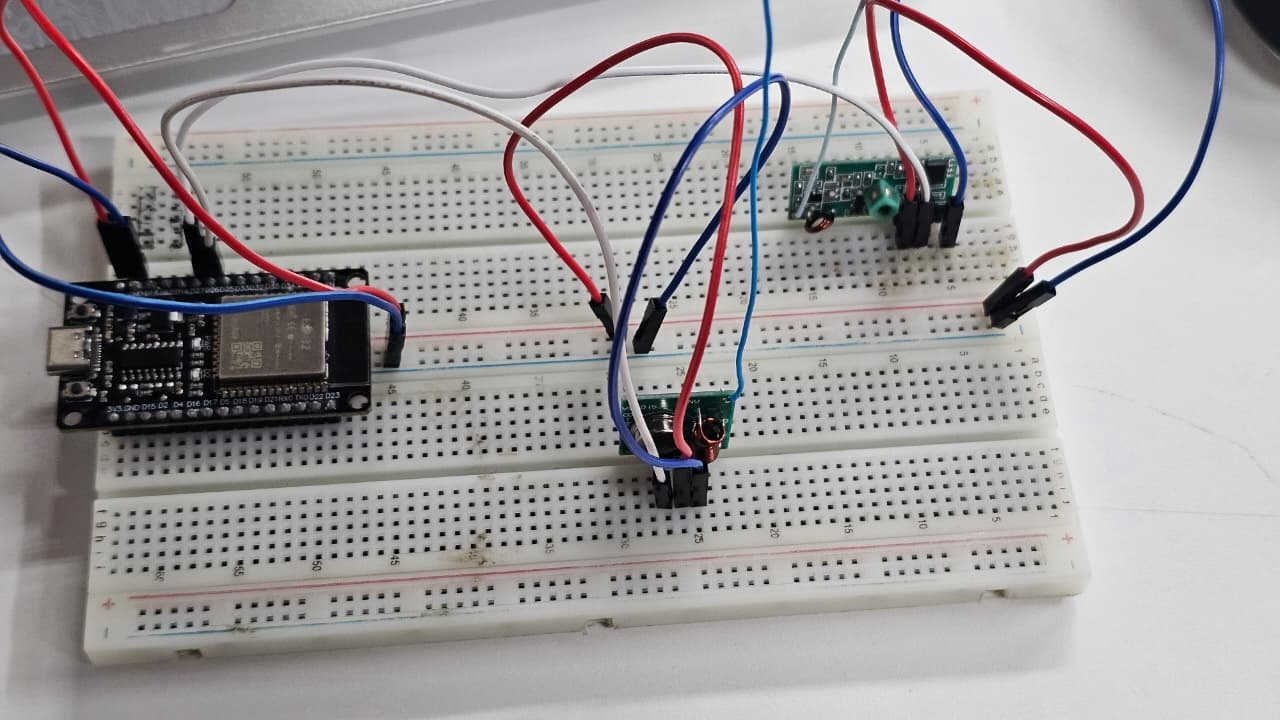
\includegraphics[width=\linewidth,height=180pt,keepaspectratio]{figuras/old_9_1.jpg}\caption{Montagem física do circuito A. Fonte: acervo da equipe.}\label{fig:old_9_1}\end{figure}
\setcounter{subsection}{3}\subsection{Circuito B — montagem}
\begin{figure}[H]
\centering
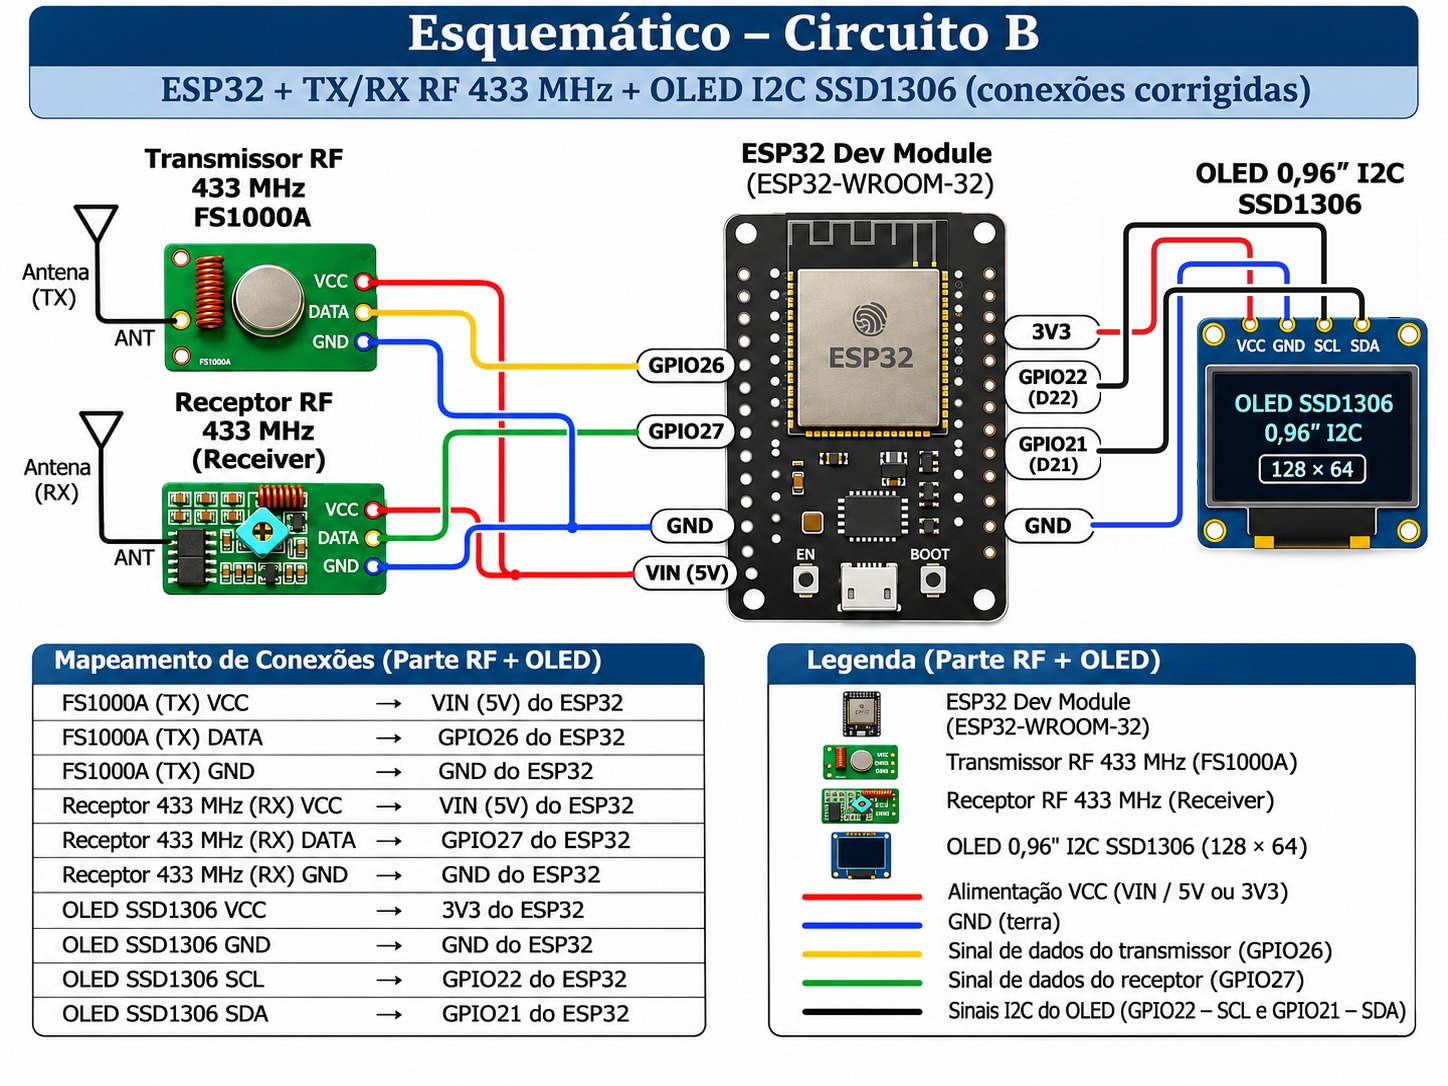
\includegraphics[width=\linewidth,height=225pt,keepaspectratio]{figuras/esq_b.png}
\caption{Esquemático atualizado do Circuito B, incluindo ESP32, módulos RF 433 MHz e display OLED SSD1306 com conexões corrigidas. Fonte: elaboração da equipe.}
\label{fig:esq_b}
\end{figure}
\begin{table}[H]\centering\small\caption{Mapeamento das ligações do circuito B}\label{tab:4}
\rowcolors{2}{tcdlight}{white}\begin{tabularx}{\linewidth}{>{\hsize=0.6186\hsize\linewidth=\hsize\raggedright\arraybackslash}X>{\hsize=1.3814\hsize\linewidth=\hsize\raggedright\arraybackslash}X}
\rowcolor{tcdnavy} \textcolor{white}{\textbf{Pino ESP32 B}} & \textcolor{white}{\textbf{Conexão}} \\
GPIO26 /\allowbreak  GPIO27 & DATA TX /\allowbreak  DATA RX, respectivamente. \\
GND & Terra comum local para TX, RX e OLED. \\
Alimentação RF & Conferir tensão e nível lógico do receptor. \\
GPIO21 /\allowbreak  GPIO22 & SDA /\allowbreak  SCL do OLED (I\textsuperscript{2}C). \\
3V3 & VCC do OLED SSD1306. \\
\bottomrule\end{tabularx}\end{table}
Repetir a montagem RF do circuito A. Acrescentar o display no barramento I\textsuperscript{2}C, alimentar o OLED em 3,3 V e ligar GND ao terra local. Conferir a ordem real dos pinos no módulo. O painel utilizado apresenta áreas amarela e azul, mas a imagem é monocromática em nível lógico.

\begin{figure}[H]\centering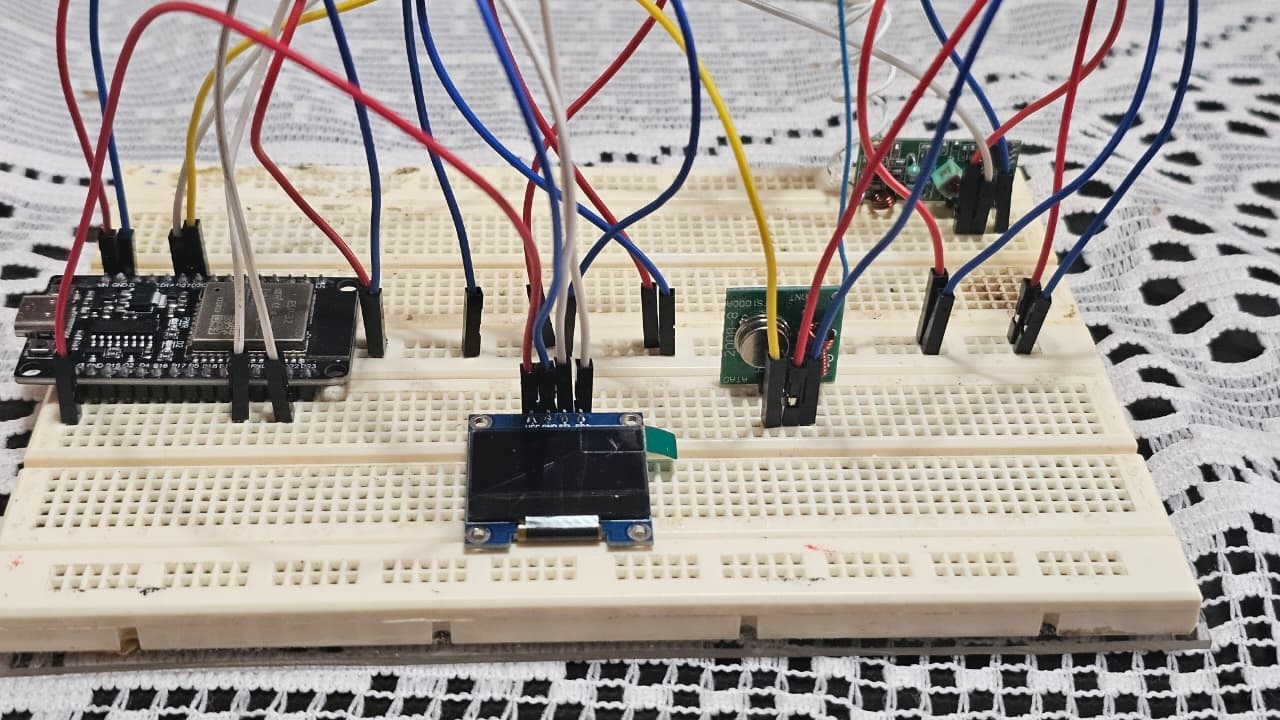
\includegraphics[width=\linewidth,height=180pt,keepaspectratio]{figuras/old_10_1.jpg}\caption{Montagem física de B com display OLED. Fonte: acervo da equipe.}\label{fig:old_10_1}\end{figure}
